\chapter{气候系统模式集合预测系统设计与实现}
\label{cha:intro}
本章先分别介绍了参数优化与初值集合方法相结合的集合预测方法BGMOPT、基于模型和观测数据融合的机器学习集合集成方法和集合预报系统的设计,然后叙述了在BCC-CSM模式上的集合预测和集合集成修正的应用案例。
\section{参数优化与初值集合相结合的集合预测方法}
利用气候系统模式做气候预测不可避免地遇到两个重要的问题是物理参数的不确定性和初值的不确定性,这两种不确定性都会给气候预测带来巨大的挑战。其中不确定参数可以通过历史试验对其进行优化。将不确定参数的个数以及参数的取值范围提供给优化算法,优化算法不断寻找使得历史试验预测结果和观测相接近的参数取值。通常此处的历史试验时间要在5年及以上,这样可以将气候中的关键气候特征如热带季节内震荡、东亚季风等模拟情况表征出来,提高模式气候模拟的整体水平。然而对于进入气候系统模式的初值来说,虽然同化方法已经尽可能降低其与真实气候情况存在的差距,但是误差不可能完全避免。又因为气候系统的混沌特性,模式对初值误差较为敏感。本文针对这两个问题,提出了一种结合参数优化的集合预测方法BGMOPT。此集合预报方法的思路如下:在重要的气候指标的指导下对气候系统模式进行参数优化,将气候系统模式的模拟性能提高到一定的基础上,然后用此改进后的模式做初值集合预报。参数优化方法利用了第二章提出的高效的基于代理模式的有约束多目标优化方法(详见算法4),初值扰动见第三章中的面向气候预测的BGM初值扰动方法。
\begin{figure}[H] % use float package if you want it here
  \centering
  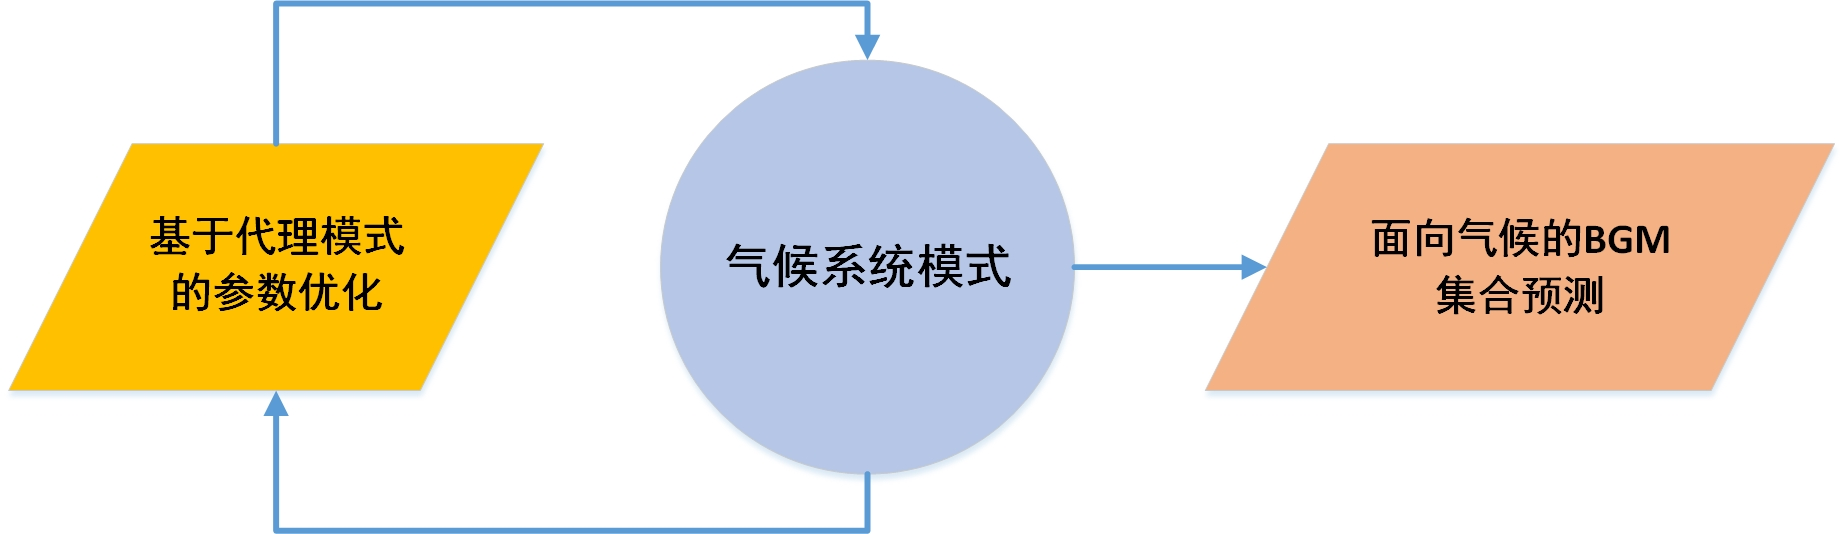
\includegraphics[scale=0.6]{figures/参数优化+初值集合.jpg}
  \caption{参数优化与初值集合方法相结合}
  \label{fig:xfig1}
\end{figure} 
\section{基于机器学习的集合集成方法}
集合预报的结果由多个集合成员共同组成,若要取得最终的确定性预报结果,则需要对集合成员的结果进行集成。本节第一小节叙述了当前确定性集合集成方法存在的不足之处,第二小节提出了基于机器学习的集合集成修正技术。
\subsection{目前集合集成方法存在的问题}
因为使用集合方法进行气候预测而导致模型运行数据大幅度增多,而当前的集合集成方法主要还是以集合平均为主,未能将如此之多的集合成员数据充分使用。且在各大气候预报中心的预报系统中通常都是多个集合成员每个月向前预报多个月,其中还有重复的模型预报数据,这些数据都是模式预测结果,一定层面上反映了模式预测的特征。图~\ref{fig:current ensem }展示了当前集合预报系统预报流程,其中output1到outputn分别为不同集合成员的输出结果。

\begin{figure}[H] % use float package if you want it here
\label{prectresult}
  \centering
  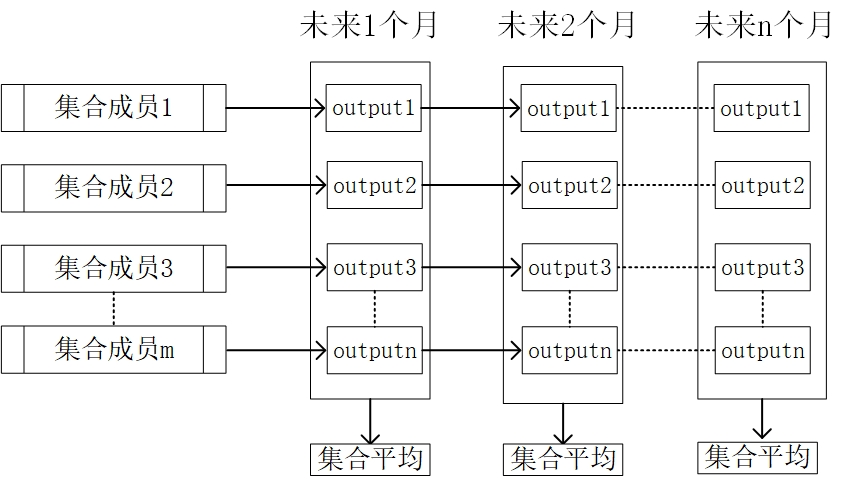
\includegraphics{figures/当前集合预报形式.jpg}
  \caption{当前集合预报形式}
  \label{fig:current ensem }
\end{figure}

\subsection{基于机器学习的集合集成修正技术}
本文接下来利用机器学习的方法设计了一种集合集成方法,此方法融合了大量的模式数据和观测数据,是对模式预测结果的集成与修正。

1. 分别为每一个起报月份,每一种lead month建立集成预测修正模型,因此修正模型个数为12个月乘以N种lead month方式共$12*n$个模型,这样做的目的是针对每个目标月不同lead month的情况对气候系统模式输出数据进行充分利用。图~\ref{fig:mlDec}展示了假设lead month为13,预测目标月为12月所需要的修正模型及其对应的输入数据。如图所示,若提前1个月起报,则已有的气候系统模式输出数据有从12月初报整个12月的数据,11月报12月的数据,10月报12月的数据,一直到前一年的12月报当前年12月的数据。图中目标月为12月份的修正模型有提前一个月起报的Model\_12m\_lead1,一直到提前13个月预测的修正模型Model\_12m\_lead13,共有13个模型,其他的预测目标月的设计依次类推。这样设计模型的思路不仅考据了不同lead month时间可用气候系统模式输出数据的不同之外,还针对不同月份设计不同的修正模型,充分利用了气候中不同年相同月份表现较为相似的特性。

2. 引入了预测当年前两年预报当月的观测数据,例如预测目标月为2018年12月,则加入2017年12月,2016年12月的观测数据也作为修正模型的输入。如果只是选取历史数据训练模型,不管往后预测到多少年,仍然不修改模型的话,则没有考虑因时间往前推进而导致的气候变化过程的因素。前两年观测数据的引入很好的结合了预报起始之前临近的气候特点。

将1和2的思想相结合,则修正模型的输入为模式数据加上临近年份的观测数据的向量,因lead month时间不同,则不同lead month对应的模型的向量长度也不同,每个修正模型的作用是构建一个由输入到输出的回归映射关系,输出为预测目标月的修正结果。而MLP模型的回归能力相比传统的线性回归等能力更高。因此每个单独的模型都由MLP组成。 

 \begin{figure}[H] % use float package if you want it here
\label{prectresult}
  \centering
  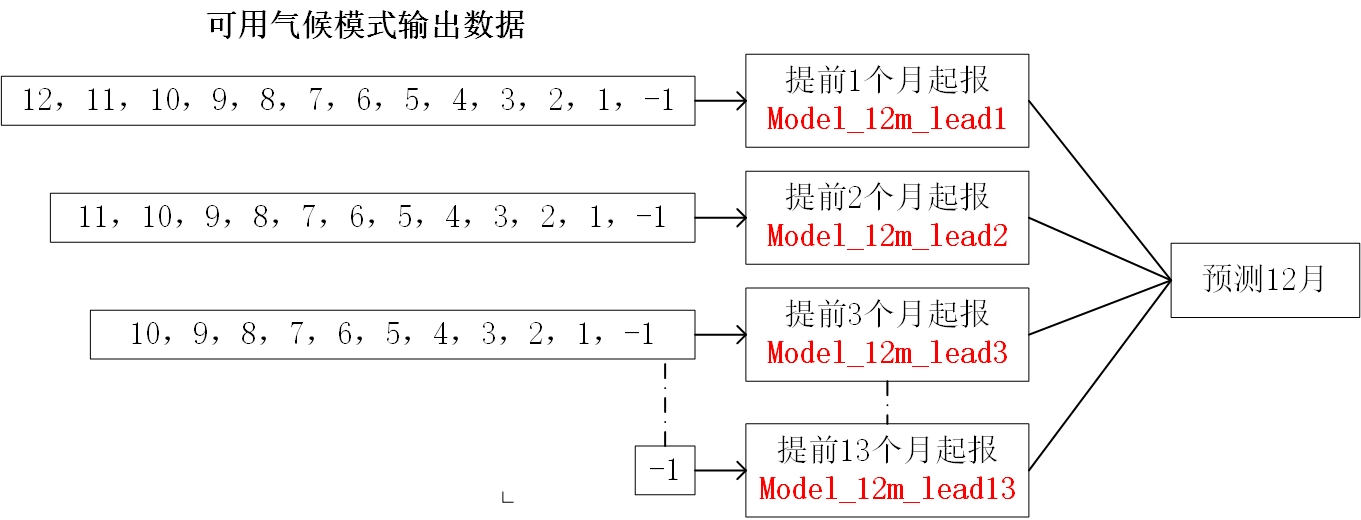
\includegraphics[scale=0.88]{figures/ML集成示意图.jpg}
  \caption{预测目标月为12月的机器学习集成修正示意图}
  \label{fig:mlDec}
\end{figure}

接下来将叙述具体的机器学习模型训练与测试过程。

(1)划分数据。首先将已有数据集划分成训练集和测试集。再将对应目标月的的模式数据抽取好,作为输入向量的一部分,将观测数据取每个目标月对应的前两年的数据抽取好作为输入向量的第二部分。

(2)初始化MLP模型。训练之前初始化所有的MLP模型。按前文所述,每一个目标月的每一种lead month分别建好初始化的模型。

(3)计算训练模型损失函数。利用所有集合成员的数据来训练MLP模型。损失函数为MLP模型输出的对应的目标月的修正结果和观测结果的RMSE。训练每一个MLP模型直至损失函数收敛。

(4)测试集成修正模型的准确率。测试数据和训练数据一样,输入为气候系统模式预测结果和临近年份的观测数据。输出为目标月气候系统模式预测结果的修正值。测试中对每一个集合成员分别用已有MLP模型进行测试,如之前的气候系统模式输出一样,这里也有对应的每一个集合成员的预测修正结果。最后将修正结果平均以得到最终的修正值。

\section{气候预测系统设计与实现}
在上述工作的基础上,本文设计了高度自动化的气候集合预测系统。系统主要包括参数优选模块、集合扰动生成模块、集合预测模块、集合集成与后处理模块和数据库模块。其结构如图~\ref{fig:forecast struct}所示。
\begin{figure}[H] % use float package if you want it here
  \centering
  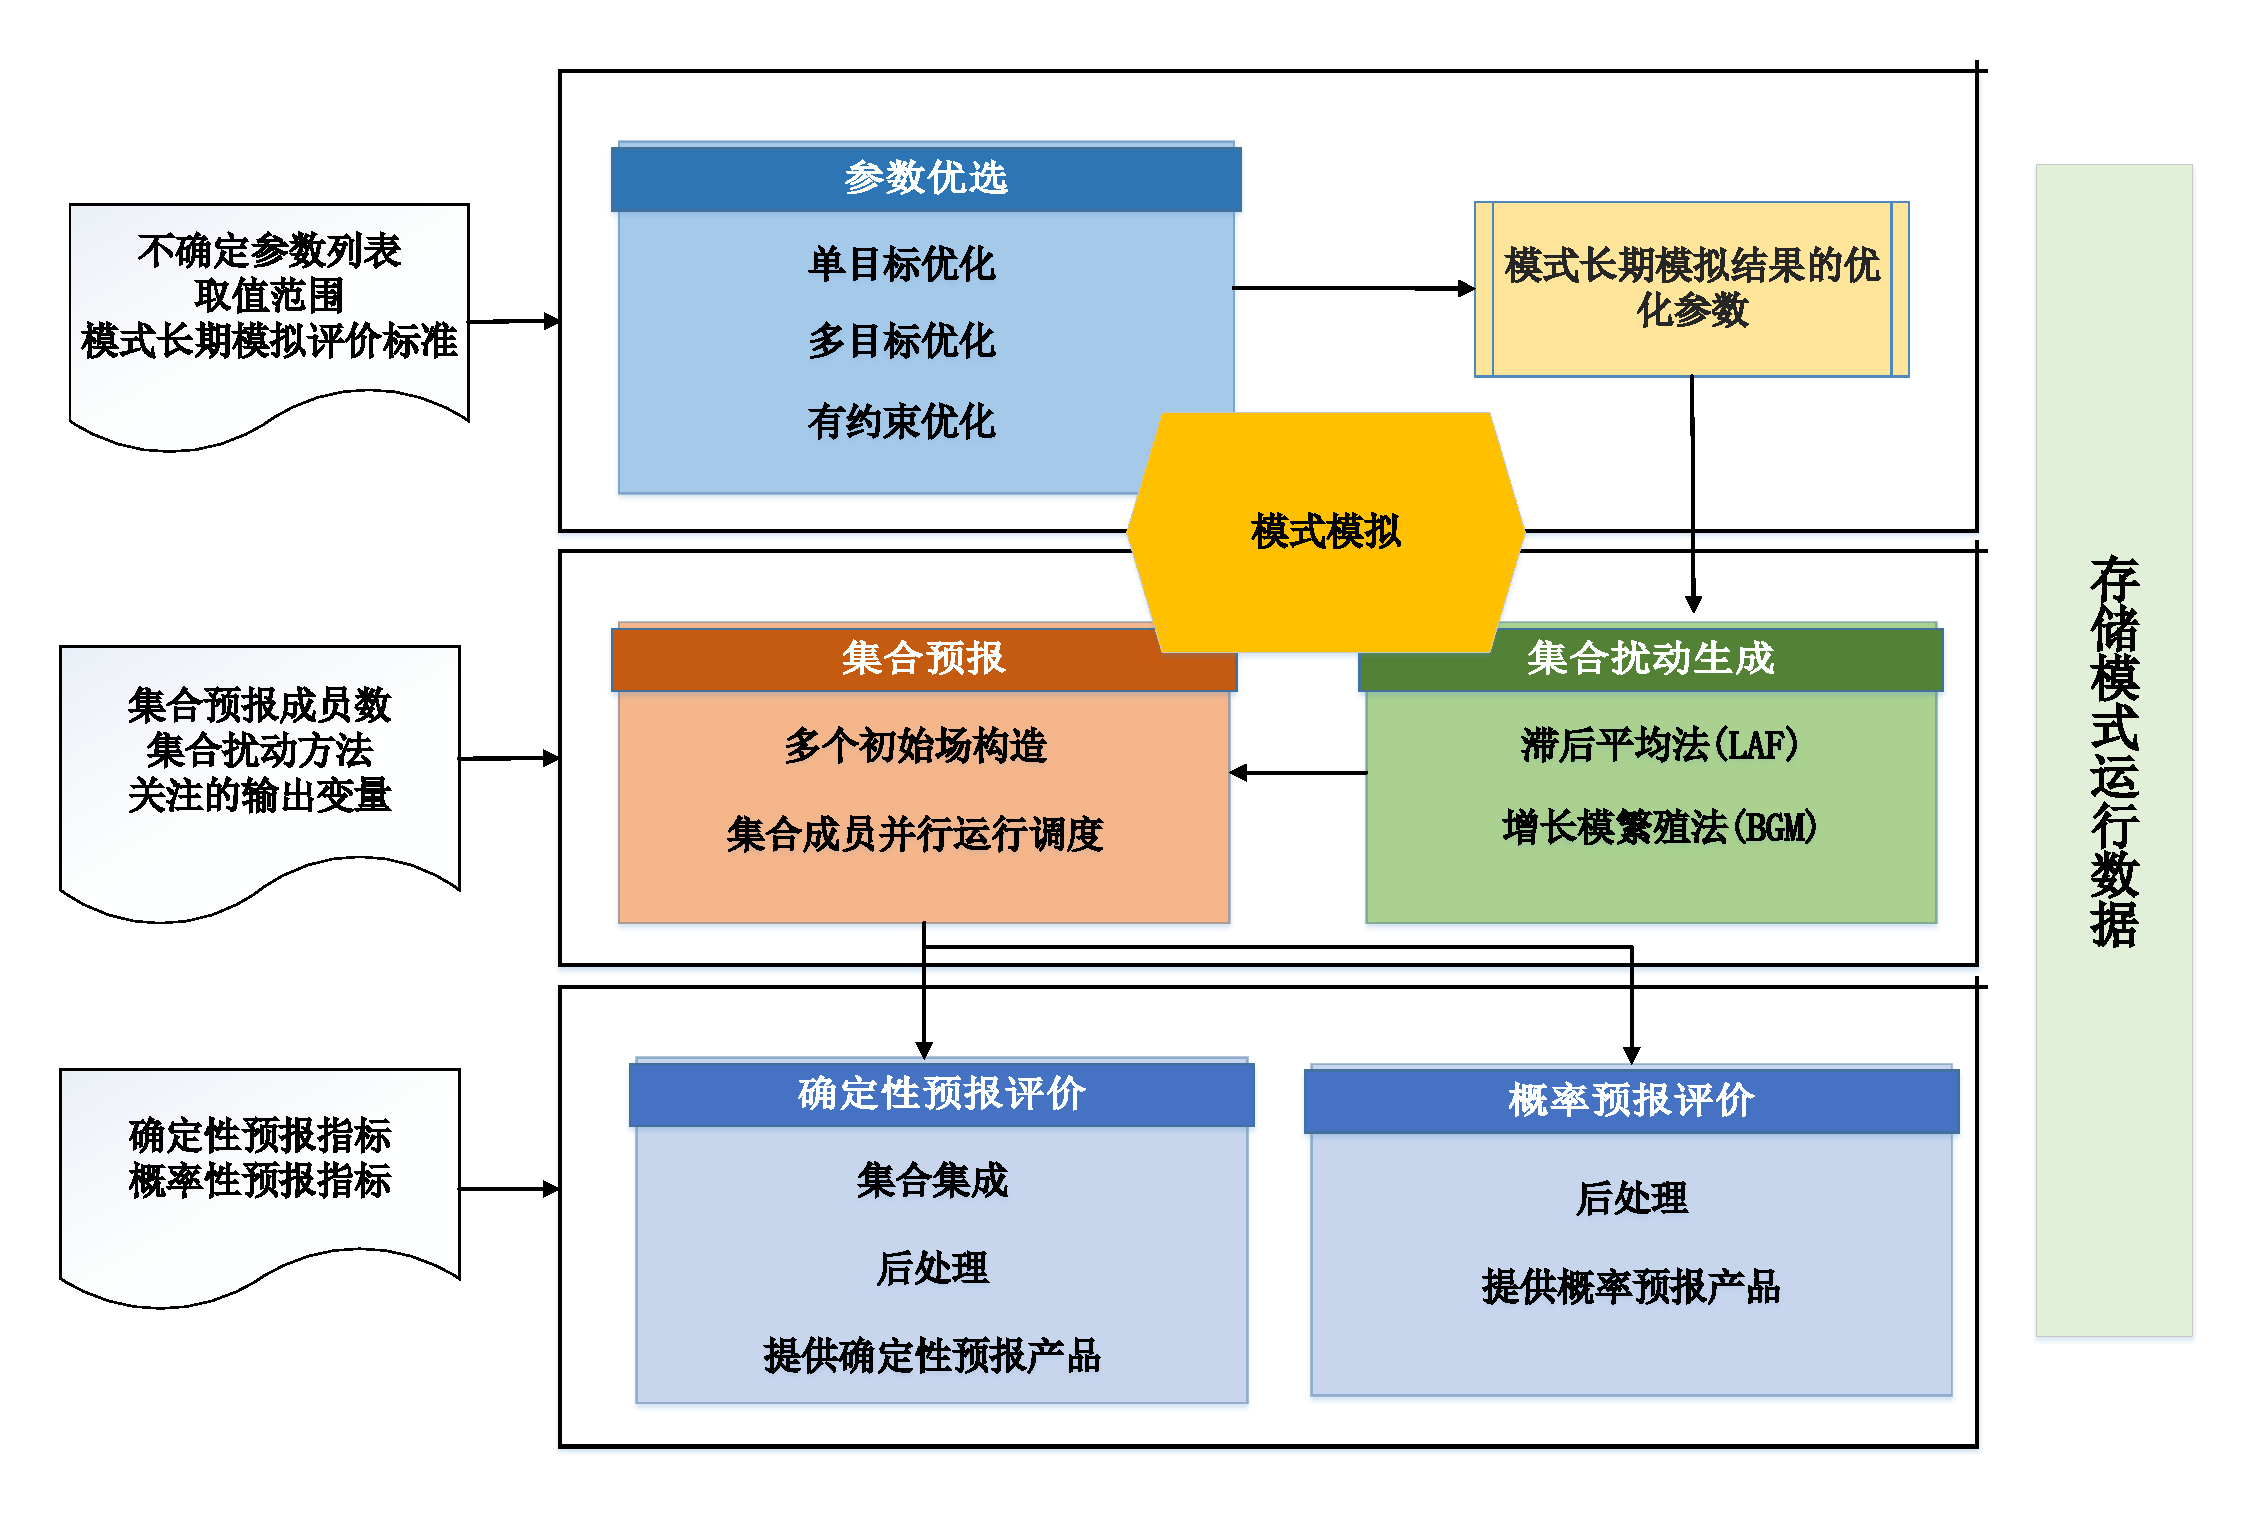
\includegraphics[scale=0.42]{figures/混合集合系统.pdf}
  \caption{集合预报系统结构}
  \label{fig:forecast struct}
\end{figure} 
1. 参数优选模块主要负责提升气候系统模式的长期气候模拟能力。它的输入为不确定参数和对应的取值范围,以及模式模拟能力评估的标准,输出为使得模式模拟能力得到提升的参数组合。它需要多次运行长期的气候系统模式来不断探索不同参数取值对模拟结果的影响。此模块中提供了一系列单目标优化、多目标优化、有约束优化的算法实现。具体实现分以下几个部分:

(1)优化问题定义部分。此部分定义问题的输入维度,参数的取值范围,所需要优化的问题等。对于气候系统模式来说,需要优化的目标是针对某一个评价标准的模式性能表现。

(2)代理模式构建部分。获取参数与其对应的气候系统模式评价结果样本时将当前所有样本用来拟合代理模式。并利用此代理模式对候选采样点进行估计。此模块包括MLP的具体拟合方法和预测方法。

(3)优化算法的优化策略部分。此部分主要是代理模式优化算法的最优样本选择策略。在单目标、多目标、有约束优化的实现过程中有些细节上的差别。

(4)优化总流程的调度。此部分将面向气候系统模式参数优化的每一个流程串联在一起,包括从一开始的拉丁超立方采样到当前真实最优采样点的计算,再到新采样点的选取等。

2. 集合扰动生成模块主要负责生成集合预测的初值扰动。本系统中提供了LAF和BGM两种方法可供选择。BGM方法相对于LAF方法在月尺度的气候预测能力上有所提升,但它获取扰动的流程相对LAF方法略为复杂。BGM方法实现由初始扰动、繁殖循环建立等部分构成。初始扰动负责在对应的扰动变量上进行所有经度、维度、垂直高度的三维扰动。繁殖循环建立包括自动化的气候系统模式提交与增长模的获取、增长率和动态调整系数的计算等过程,具体细节如第三章所述。LAF方法实现相对简单,在获取滞后天数的取值之后,系统将会自动按LAF方法更改所有集合成员模式运行所需设置的起始日期和初始场信息等。

3. 集合预测模块主要负责并行进行气候系统模式气候模拟试验。此模块的输入是集合扰动模块所提供的扰动。集合预测将扰动和初始场相叠加则形成扰动场,利用Shell脚本自动调度扰动实验和控制实验的并行提交和运行。

4. 集合集成与后处理模块主要有确定性和概率性集合后处理和评价方法。其中确定性集合集成方法包括传统的集合平均以及基于机器学习的集合集成技术。机器学习的集合集成方案如第四章所述,它的使用只需要输入目标月和lead month以及气候系统模式输出数据和观测数据的位置等信息,系统会自动进行以下步骤:

(1)根据目标月和lead month,自动选择对应的集成修正模型。

(2)处理气候系统模式的输出结果和观测数据获取输入向量。

(3)利用集成修正模型获取更加准确的集成结果。确定性集合评价方法本系统提供了时间相关系数,均方根误差,均方误差等评价标准。概率性评估暂时只提供了常用的Brier评分方法。

5. 数据库模块主要用于记录气候系统模式的运行记录。每一次参数优化和集合结果将被保存到数据库,以备后续进一步对气候系统模式的研究与分析。

\section{面向BCC-CSM气候系统模式的集合预测案例试验}
针对降水预测在气候系统模式中的预测相对较为困难的情况,本节将详细叙述在BCC-CSM耦合气候系统模式上提升降水预测能力的应用。首先利用多目标约束参数优化算法对BCC-CSM气候系统模式中的不确定参数进行调整,使得模式对影响降水的气候特征的模拟能力上升。然后在优化参数后的气候系统模式上做BGM初值集合预测,最后将此集合预测案例试验结果与LAF集合方法预测结果进行对比。
\subsection{BCC-CSM气候系统模式不确定参数优化}
对于BCC-CSM模拟降水而言,热带大气季节内振荡 (Madden-Julian oscillation,MJO)和东亚夏季风(The East Asian summer monsoon, EASM)的气候特征备受关注。其中MJO源于热带地区,为30至60天的准周期性季节内振荡,以热带地区对流增强/减弱区向东传播为主要特征,是次季节到季节尺度上预测的重要部分~\cite{梁萍2013mjo}。它不仅对低纬度地区气候预测有较强的影响,还通过经向传播和遥相关对高纬度地区的气候预测有一定的影响~\cite{任宏利2015mjo}。研究表明,MJO作为全球最强低频信号,对全球降水有明显的影响~\cite{mo1998tropical},另外MJO对我国降水有着不可忽略的重要意义~\cite{白旭旭2011mjo,吴捷2018mjo}。

EASM对世界人口最多的东亚地区的降水有着关键影响。我国正是典型的季风影响区,EASM对我国的夏季降雨有着重要的意义~\cite{王会军2013东亚季风近几十年来的主要变化特征}。研究表明在受夏季风影响的我国东部区域的夏季降水占到全年降水的49\%,可以说东亚夏季风在一定程度上决定着我国的水资源分布~\cite{周天军2018东亚夏季风变化机理的模拟和未来变化的预估}。

上述两个重要的气候现象对降水意义重大,提升其模拟能力对BCC-CSM气候系统模式来说十分重要。但是在BCC-CSM模式的深对流、浅对流和云等参数化方案中存在一系列的不确定性参数,这些参数的默认值在模式发布时给出,由气候专家建议其取值范围,对MJO和EASM模拟能力影响巨大。因此本节针对MJO和EASM这两个重要的气候指标对不确定参数进行调整。另外为了保证BCC-CSM耦合模式的能量守恒,不因调整不确定参数而导致模式无法无法长期稳定运行,因此本文不仅利用MJO和EASM这两个指标,还结合了模式顶辐射平衡约束对BCC-CSM长期的耦合模拟中不确定参数进行校正,参数优化试验的气候模拟时长为6年,后五年的模拟结果用来评估模拟性能。不确定参数列表如表~\ref{tab:bccparam}所示。

\begin{table}[H]
\centering
\caption{BCC-CSM大气模块待调整的参数及其范围}  
\begin{tabular}{llll}  
\toprule[1.5pt]
\centering
参数名称 & 参数含义 &默认值  & 取值范围 \\  
\hline  
 ke & 深对流降水蒸发参数 & 1.00E-06 & 5.00E-07~1.00E-05 \\
    c0 & 云水转换为雨水的转换率 & 2.00E-03 & 1.00E-03~6.00E-03 \\
    conv\_RH\_threshold & 对流触发相对湿度阈值 & 0.7   & 0.6~0.85 \\
    bottposit\_convclouds
 & 控制对流云云底位置的参数 & 650   & 550~750 \\
    cmftau & 浅对流时间调整尺度 & 1800  & 900~9000 \\
    c0 & 浅对流雨水转换率 & 8.00E-05 & 1.00E-05~5.00E-04 \\
    rhminl & 低云相对湿度阈值 & 0.945 & 0.65~0.99 \\
    rhminh & 高云相对湿度阈值 & 0.87  & 0.65~0.99 \\
    ricru & 控制边界层高度参数 & 0.39  & 0.25~0.5 \\
    conke & 控制大尺度降水蒸发的参数 & 1.00E-05 & 1.00E-06~1.00E-04 \\
    icritc & 冷冰转换阈值 & 8.00E-06 & 1.00E-06~1.00E-04 \\
    icritw & 暖冰转换阈值 & 4.00E-04 & 1.00E-04~5.00E-04 \\
    r3lcrit & 液水转换半径阈值 & 1.20E-05 & 5.00E-06~1.50E-05 \\
    cloud\_effecradius\_para\_A
 & 云滴有效半径阈值 & 3 & 1~5 \\
   cloud\_effecradius\_para\_B
 & 云滴有效半径阈值 & 25 & 15~40 \\
\bottomrule[1.5pt]  
\end{tabular} 
\label{tab:bccparam}
\end{table}

接下来将介绍MJO和EASM评价标准设计以及辐射平衡约束定义。MJO评价方法主要关注信号的传播和周期。本文这里设计了三个分量指标如表~\ref{tab:mjometrics}所示。
\begin{table}[H]
\centering
\caption{MJO指标设计}  
\begin{tabular}{lll}  
\toprule[1.5pt]
\centering
No. & 指标名 & 物理意义  \\  
\hline  
    1        & $sc\_w$    & 冬季U850和OLR波谱分析场的次季节尺度东传波谱占比模拟能力 \\
    2        & $sc\_s$ & 夏季U850和OLR波谱分析场的次季节尺度东传波谱占比模拟能力 \\
    3        & $sc\_l$    &基于U850和OLR的8位相合成,模拟与观测的相关 \\
\bottomrule[1.5pt]  
\end{tabular} 
\label{tab:mjometrics}
\end{table}

MJO综合评分公式为:
\begin{equation}
\label{mjoeq}
 mjo\_score =  \frac {sc\_w + sc\_s + sc\_l}  {3.0}   
\end{equation}
其中$sc\_w$是表征冬季次季节信号的模拟能力,$sc\_s$表征对夏季次季节信号的模拟能力,$sc\_l$表征MJO向东传播的模拟能力,它们的值越大代表模拟能力越强。

东亚季风评价方法主要关注季风爆发的进程,指标设计如表~\ref{tab:easmmetrics}所示。
% Table generated by Excel2LaTeX from sheet 'Sheet1'
\begin{table}[H]
\centering
\caption{EASM指标设计}  
\begin{tabular}{lll}  
\toprule[1.5pt]
\centering
No. & 指标名 & 物理意义  \\  
\hline  
    1        & $onset$    & 季风爆发侯(降水量超过月平均值5mm/day的第一侯) \\
    2        & $withdraw$ & 季风撤退侯(降水量超过月平均值5mm/day的最后一侯) \\
\bottomrule[1.5pt]  
\end{tabular}  
\label{tab:easmmetrics}
\end{table}

综合评分$easm\_score$公式如下所示:
\begin{equation}
ccr = \frac {onset + withdraw} {2.0}    
\end{equation}
\begin{equation}
easm\_score = {ccr} * \operatorname sqrt  (\frac {  df  }  {1 - \operatorname  ccr  ^  2})    
\end{equation}
$easm\_score$为$ccr$相关系数的显著性检验t值,其中$df$为有效格点数的自由度。t值越大代表显著性越明显,相关性越可靠。

模式顶辐射平衡的定义为模式顶净短波辐射(FSNT)和净长波辐射(FLNT)的绝对值之差小于1W/m$^2$.

因此最大化MJO和EASM评分并保证大气顶辐射平衡的多目标约束优化问题可以定义为:
\begin{equation}
\begin{cases}
 \max_{{x}} F({x},mjo\_score(x),easm\_score(x)) \\
      \text{subject to:} \\
       \qquad  ABS(FSNT(x)-FLNT(x)) - 1  <  0
\end{cases}
\end{equation}

采用第2章中提到的多目标约束优化方法对BCC-CSM气候系统模式进行参数优化,得到的结果如表~\ref{bccoptresult}所示。结果表明在满足辐射平衡约束的基础上,优化参数后的模型在MJO模拟效果上相对于默认实验改进十分明显。而东亚季风相对于默认实验也有一定程度的改进。
\begin{table}[H]
\label{table:reslutofBCC}
\centering
\caption{BCC-CSM长期模拟改进结果}  
\begin{tabular}{llll}  
\toprule[1.5pt]
\centering
  & mjo\_score & easm\_score  & radiation bias\\  
\hline  
    exp      & 1.65     & 5.741047 & 0.4577 \\
    cntl     & -0.1182  & 5.6985   & 0.392997 \\
\bottomrule[1.5pt]  
\end{tabular}  
\label{bccoptresult}
\end{table}
为了显示MJO模拟能力提升的效果,下面将展示MJO东传信号的8位相合成图和冬季u850波谱场。

\begin{figure}[H] % use float package if you want it here
  \centering
  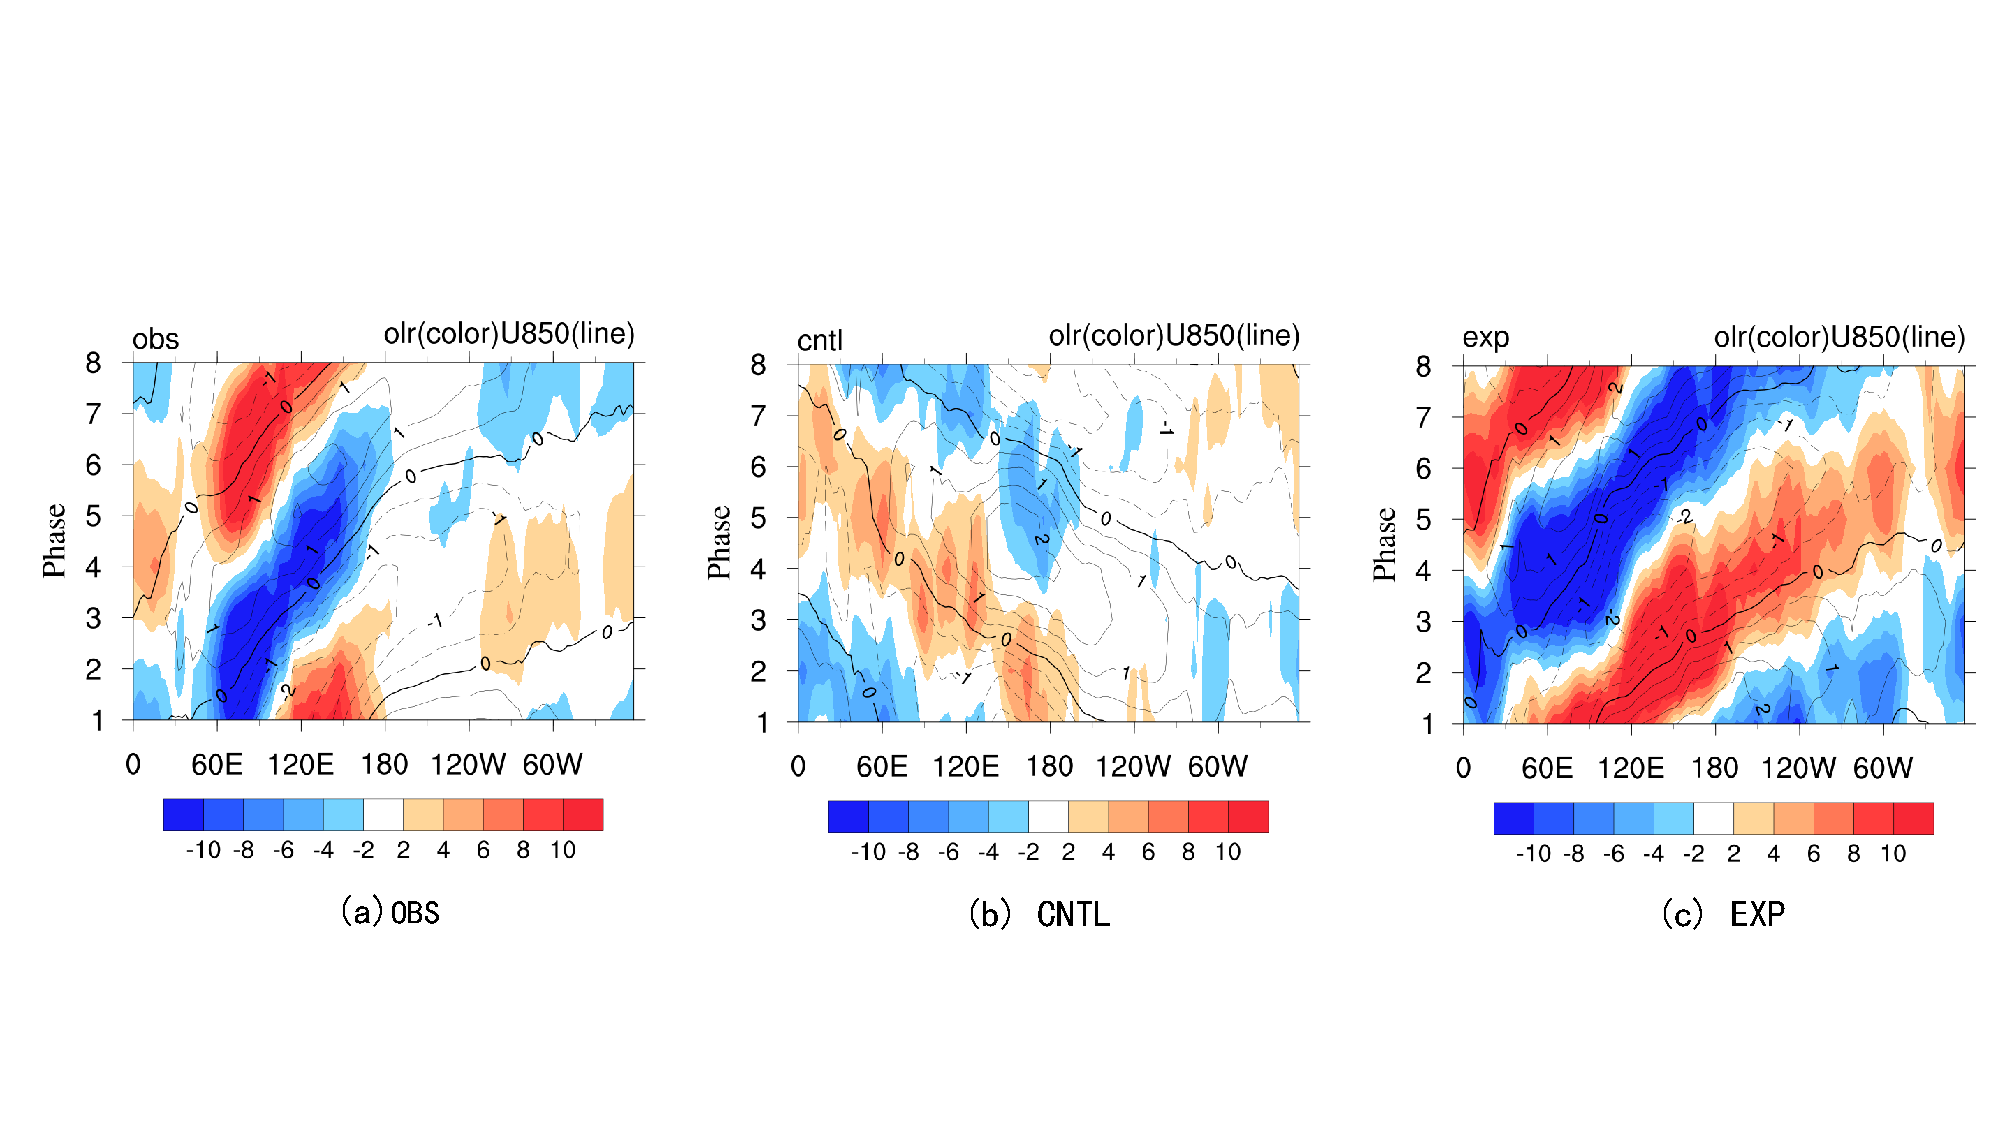
\includegraphics[scale=0.46,trim=20 85 10 150,clip]{figures/phase.pdf}
  \caption{MJO信号8位相合成图结果对比}
  \label{fig:mjo phase}
\end{figure}

\begin{figure}[H] % use float package if you want it here
  \centering
  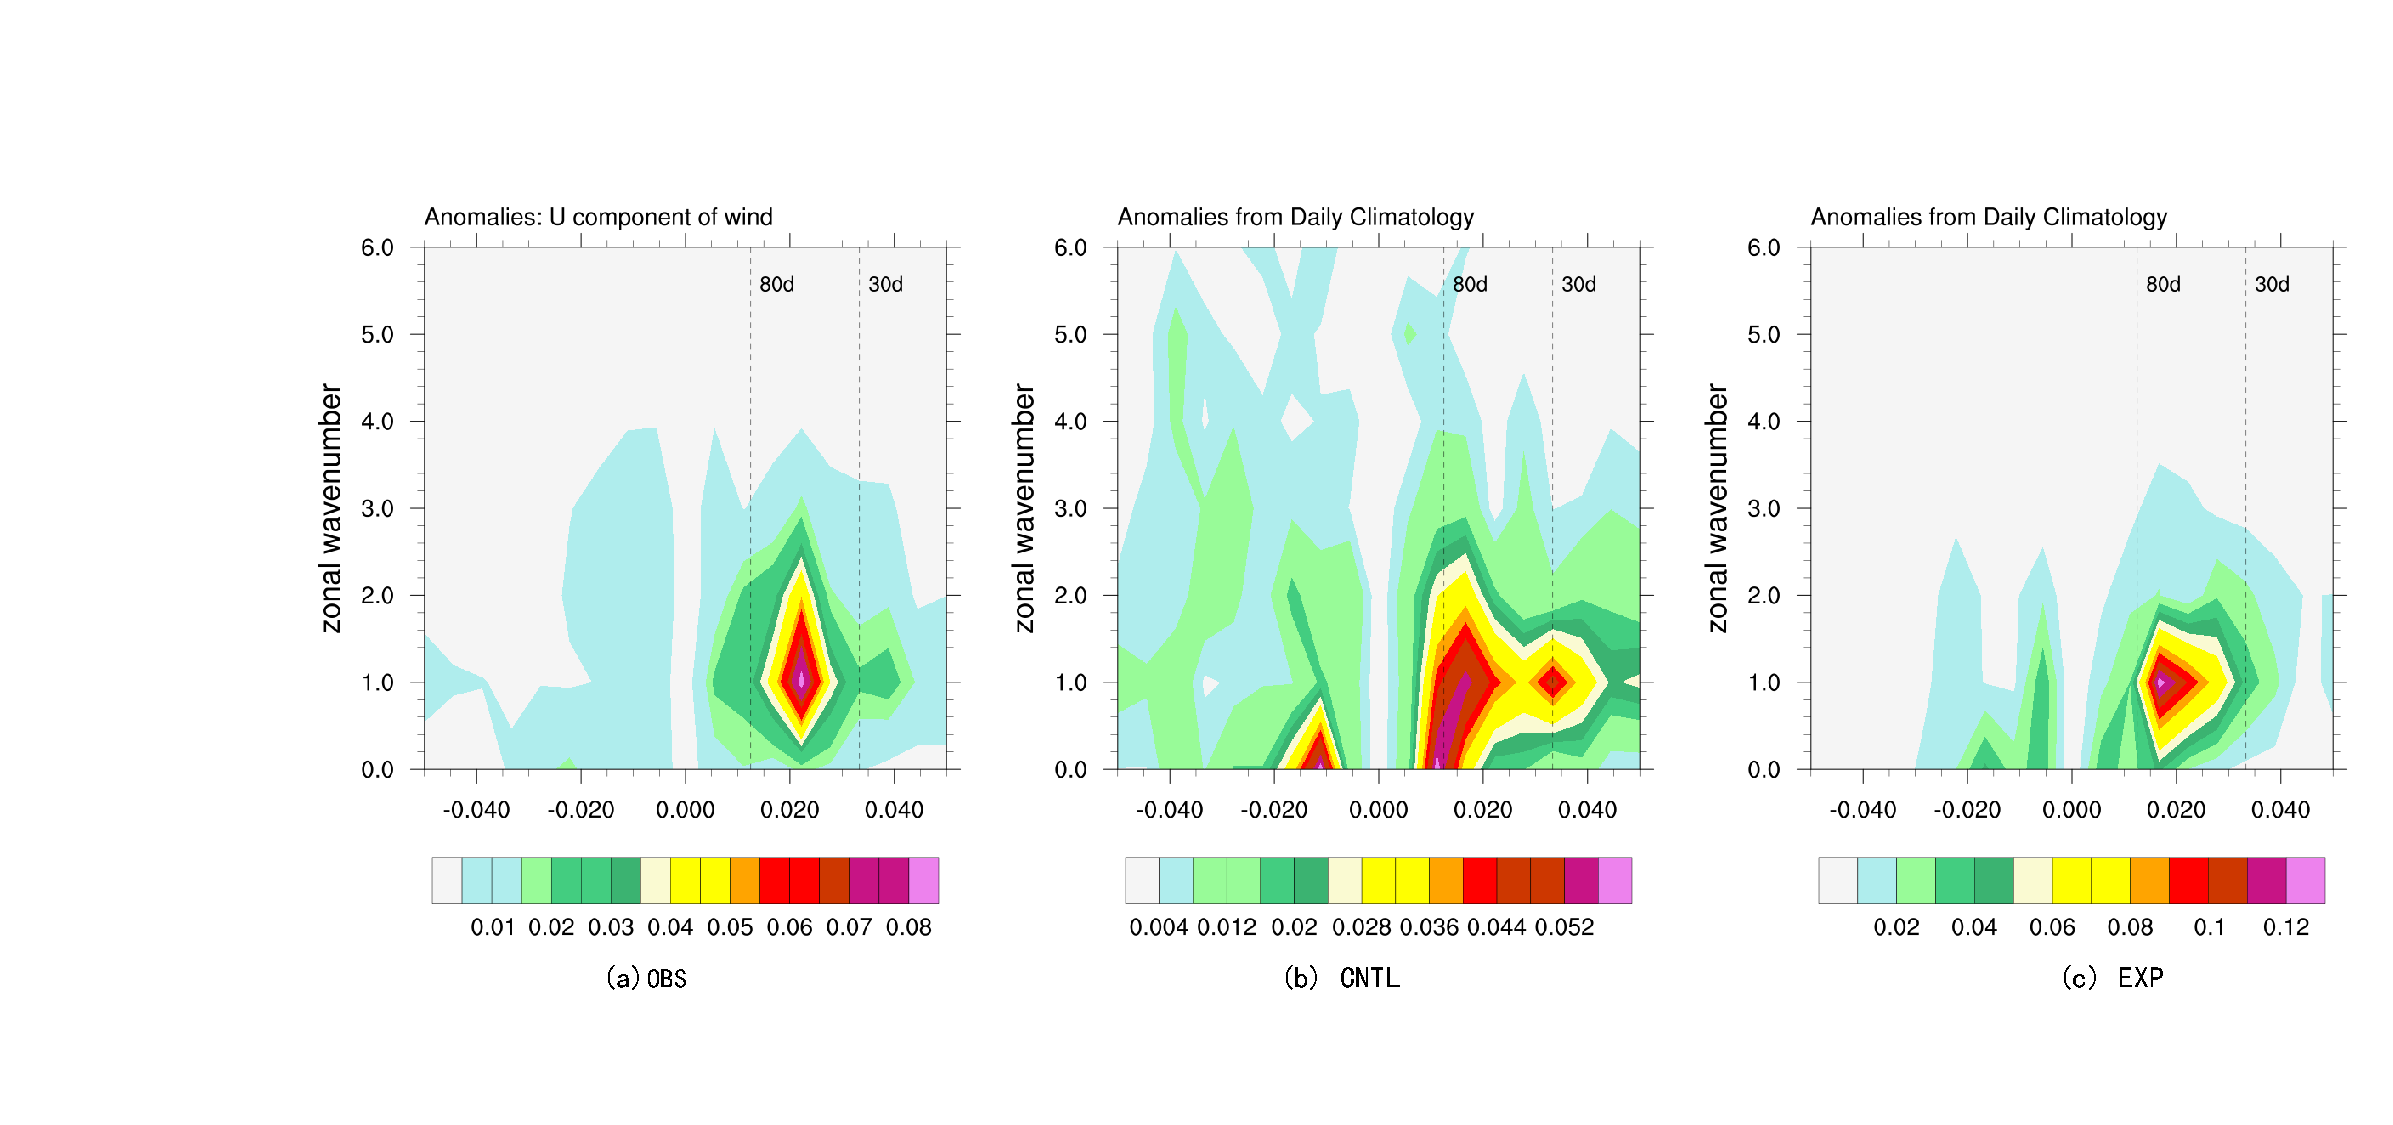
\includegraphics[scale=0.45,trim=155 50 20 110,clip]{figures/u850-winter3.pdf}
  \caption{冬季U850波谱场模拟效果对比}
  \label{fig:mjo u850}
\end{figure}
从图~\ref{fig:mjo phase}和~\ref{fig:mjo u850}可以看出,默认实验(CNTL)对MJO的模拟能力很弱,而改进参数后的模拟结果(EXP)与观测(OBS)的MJO信号更为接近。

EASM登陆和退出的进程模拟结果见图~\ref{Fig:easmresut}所示。对比默认实验,改进的模型对东亚季风的登陆过程有更强的模拟能力,而退出进程却相对较差。由于登陆进程相对默认实验改进17\%,退出进程变差的百分比只有6\%。所以整体东亚季风的模拟能力还是相对较好的。

综上所述,在BCC-CSM气候系统模式中经过物理参数的优化,5年历史试验的辐射平衡满足条件,且MJO和东亚季风的模拟能力相对默认实验进一步增强,至此BGMOPT完成第一阶段的物理参数优化工作。

\begin{figure}[H] % use float package if you want it here
 \centering
 \subfigure[观测的东亚夏季风进程]{
 \centering
    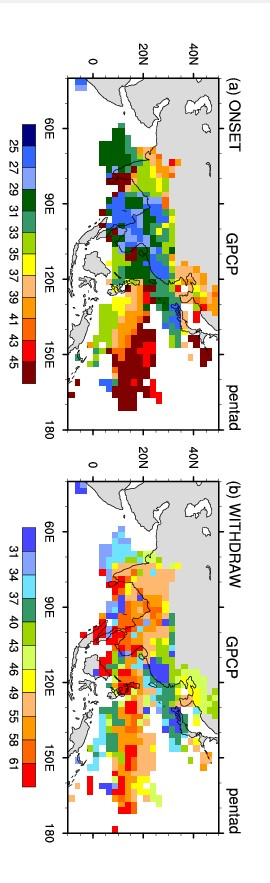
\includegraphics[angle=90,trim=0 15 0 15,clip]{obs_easm.png}
 }

 \subfigure[控制实验的东亚夏季风进程]{
 \centering
     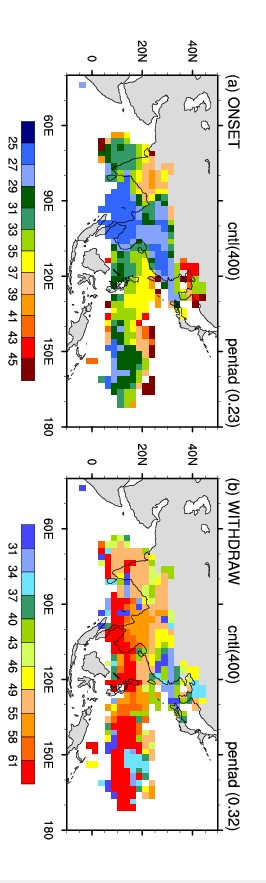
\includegraphics[angle=90,trim=0 15 0 15,clip]{cntl_easm.png}
 }
 \subfigure[改进参数后的东亚夏季风进程]{
 \centering
     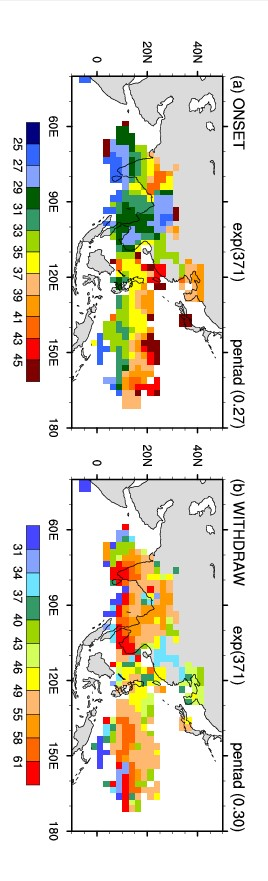
\includegraphics[angle=90,trim=0 15 0 15,clip]{opt_easm.png}
 }
\caption{EASM模拟结果对比}
\label{Fig:easmresut}
\end{figure}


\subsection{BCC-CSM气候系统模式集合预测结果分析}
将上述优化参数带入BCC-CSM气候系统模式开展初值集合实验。初值集合回报试验设置的时间为2008年12月1日至2009年3月31日。BGMOPT初值扰动实验开始的时间为2008年11月11日。集合成员为4对正负扰动实验和一个控制实验,共9个集合成员。同样,这里也将BGMOPT与LAF集合方法做了对比。LAF的滞后时间也同样是3天,集合预报由8个滞后扰动实验和一个控制实验,共9个集合成员组成。

下文将叙述本章提出的集合方法相对于国家气候中心所使用的LAF方法的预测技巧的对比结果。预测技巧用均方误差和相关性的比较结果来衡量。

假设有A集合和B集合预测结果,它们的均方误差相比结果如下公式中的$MSE\_ratio$所示。其中$I$为总格点数,$w ( i ) $为网格权重,$X _ { \mathrm { A } } ( i )$为A集合在$i$格点的预测结果,$X _ { \mathrm { o} } ( i )$为观测在$i$格点的预测结果$X _ { \mathrm { B } } ( i )$为B集合在$i$格点的预测结果。相关性比较correlation ratio的计算也与此类似。$MSE\_ratio$小于1则A集合比B集合预测结果更好,correlation ratio大于1则A集合比B集合预测结果更好。
\begin{align}
& MSE_A = \sum _ { i = 1 } ^ { I } w ( i ) \left( X _ { \mathrm { A } } ( i ) - X _ { \mathrm { o } }  ( i ) \right) ^ { 2 }  \\
& MSE_B = \sum _ { i = 1 } ^ { I } w ( i ) \left( X _ { \mathrm { B } } ( i ) - X _ { \mathrm { o } }  ( i ) \right) ^ { 2 }  \\
& MSE\_ratio = \frac {MSE_A}{MSE_B} \label{eq:MSE}
\end{align}

从图~\ref{fig:prect bgmopt}中可以看出,起报后的四个月中BGMOPT相对于LAF方法在降水预测的均方误差方面的改进分别为11.4\%、16.9\%、12.2\%、19.9\%,平均改进为15.1\%。而对于相关系数而言,BGMOPT方案在lead 3 和lead 4月份内也相对LAF方法有所变好。其他月份内的相关系数虽略有变差但也都与原方法的相似度在95\%以上。因此可以总结本章提到的集合方案在BCC-CSM模式的试验案例中对降水模拟有明显的提高。

\begin{figure}[H] % use float package if you want it here
\label{prectresult}
  \centering
  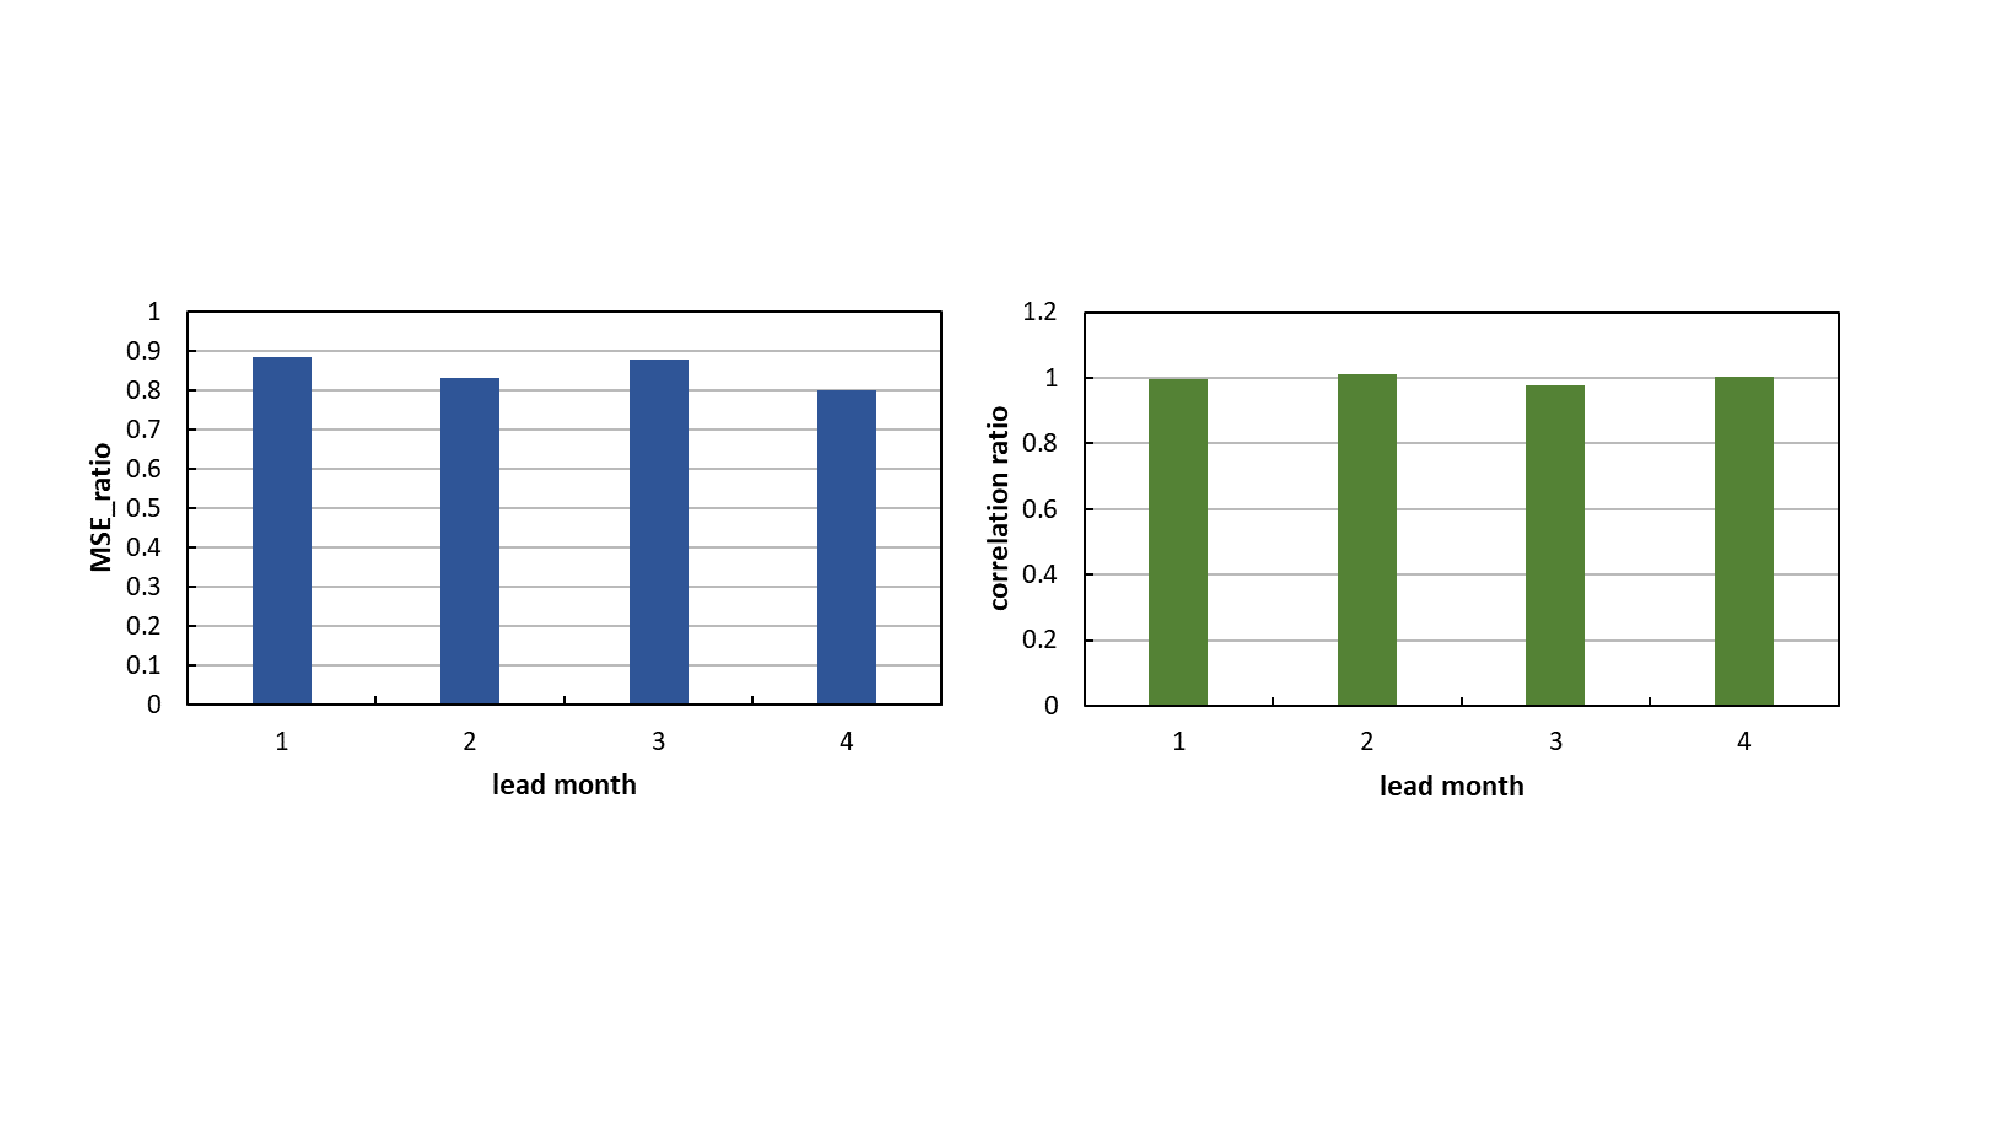
\includegraphics[scale=0.50,trim=0 125 0 125,clip]{figures/BGMOPTPRECT1.pdf}
  \caption{BGMOPT相比LAF集合方法对降水模拟的改进结果}
  \label{fig:prect bgmopt}
\end{figure}

另外为了兼顾大部分季节预测的关键变量在此过程中的变化,除了降水之外,下面还将展示BGMOPT和LAF集合方法的850hpa温度、850hpa纬向风、200hpa纬向风、850hpa径向风、500hpa位势高度和地表温度(观测见第三章中的表~\ref{tab:eva varibles})在起报的1、2、3、4(图~\ref{fig:rmse bgmopt allvar},~\ref{fig:coef bgmopt allvar}中变量的下标分别是l1、l2、l3、l4)个月内的标准偏差和相关系数。由图~\ref{fig:rmse bgmopt allvar}可以看出BGMOPT集合方法所预报的大部分变量在整个季节预报内都相对于LAF方法有明显改进,特别是850hpa温度、降水和地表温度。同样在相关系数方面本文提出的方法和原方法十分相似,只有V850变量有明显的改进。

\begin{figure}[H] % use float package if you want it here
\label{prectresult}
  \centering
  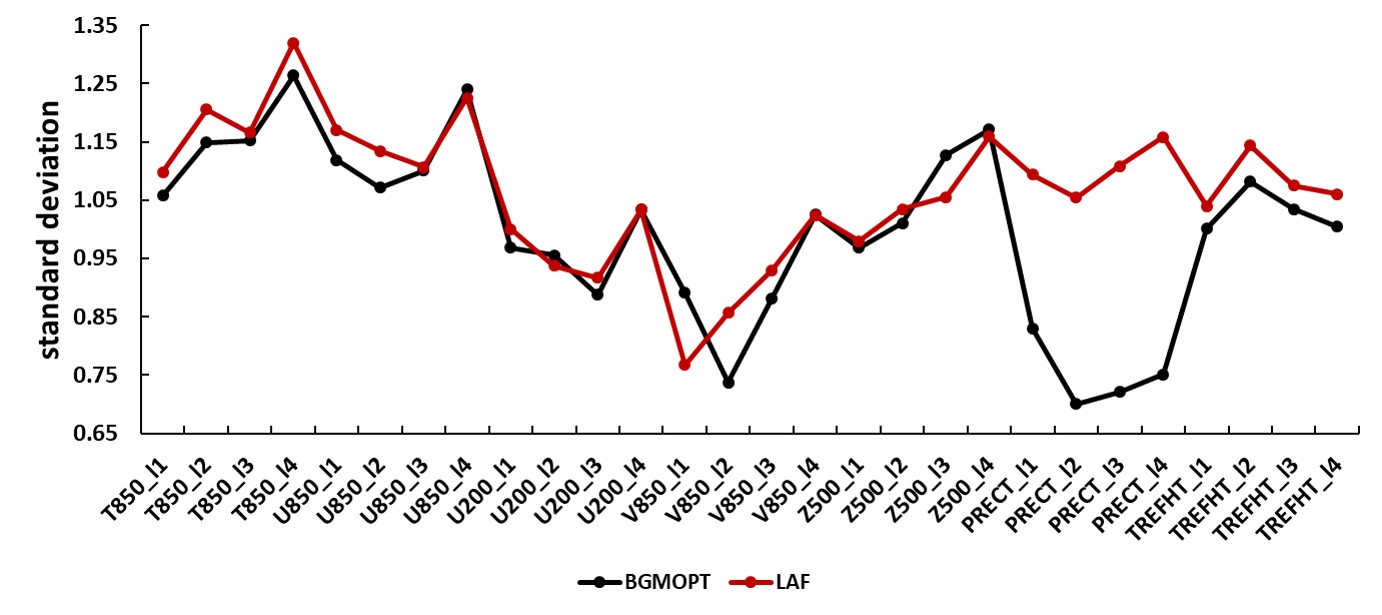
\includegraphics[scale=0.6]{figures/allvar-std.jpg}
  \caption{集合方法针对降水标准偏差结果对比}
  \label{fig:rmse bgmopt allvar}
\end{figure} 

\begin{figure}[H] % use float package if you want it here
\label{prectresult}
  \centering
  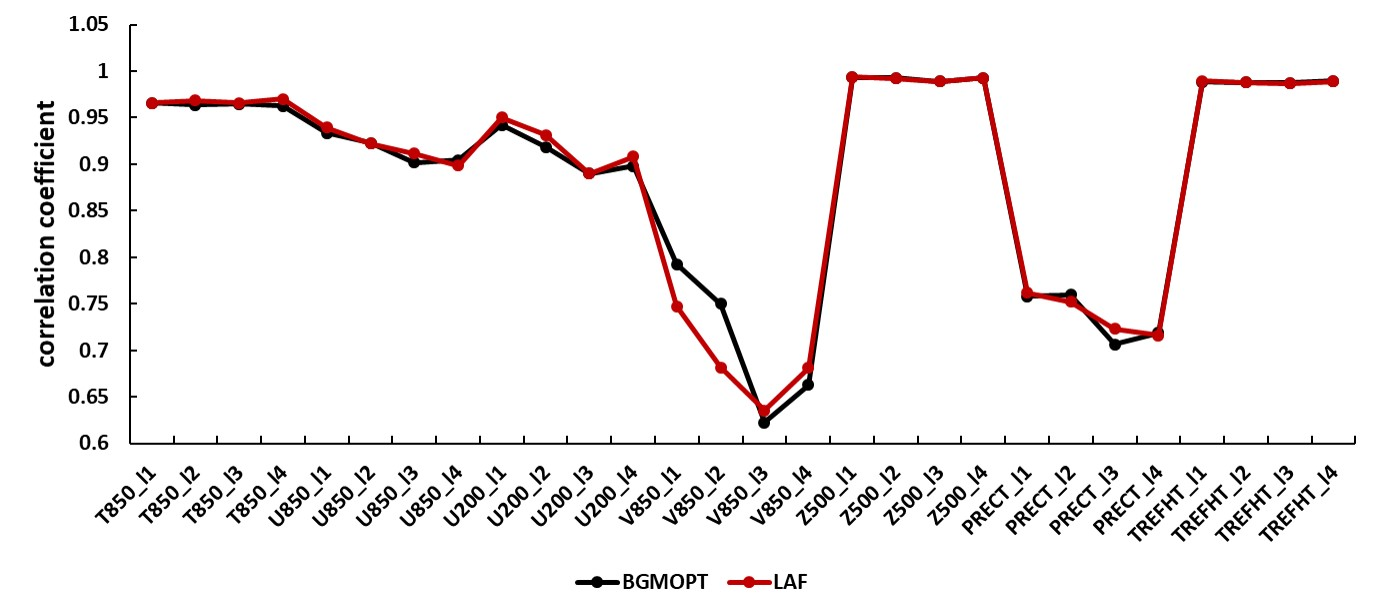
\includegraphics[scale=0.6]{figures/allvar_coef.jpg}
  \caption{集合方法针对降水相关系数结果对比}
  \label{fig:coef bgmopt allvar}
\end{figure} 

综上所述,本章提出的结合参数优化的初值集合方法对BCC-CSM短期气候降水模拟技巧有显著的提升,与此同时大部分其他重要的短期气候预测变量都略有变好。
%\begin{figure}[H] % use float package if you want it here
%  \centering
%  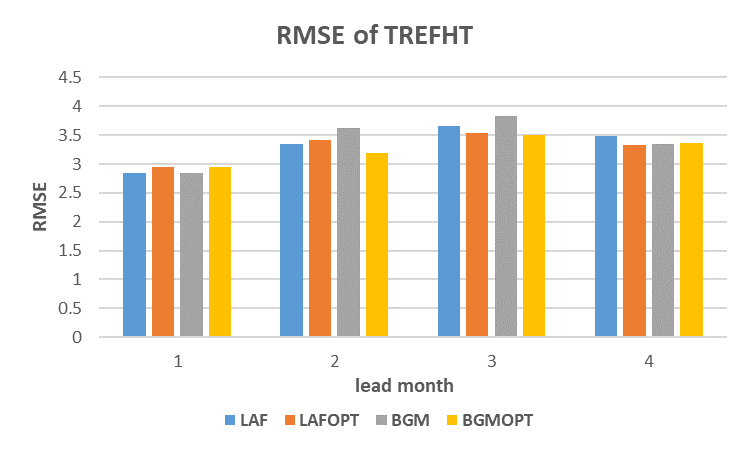
\includegraphics{figures/RMSE_TREFHT1.png}
%  \caption{TREFHT结果对比}
% \label{fig:xfig1}
%\end{figure} 
\subsection{BCC-CSM气候系统模式预测回报试验的集合集成结果分析}
ENSO是全球尺度的振荡现象,海气相互作用的显著事件,对全球大规模和局地小规模的气候异常关系密切~\cite{任福民2012近}。目前对它的预报主要通过NINO3或NINO3.4区的区域平均海平面温度(SST)来判定。若要提高ENSO的预报能力,进一步提高SST预测的准确性十分关键。但是目前集合集成方法简单,大量模式数据和观测数据未能融合使用,针对此问题,本小节使用4.2节中提出的集合集成修正方法对lead month为13个月,集合成员数目为24的BCC-CSM气候系统模式集合预测SST结果进行集合集成。
按照前文所述,此处建立了156(12月*13 lead month)个MLP模型,每个模型为4层MLP全连接神经网络。

训练数据为1995年-2003年的模式数据和前两年对应目标月的观测,测试数据为2004年-2017年的模式数据和观测。测试数据集合成员的利用是将每一个集合成员经过修正模型修正后得到修正结果。24个集合成员的平均修正结果作为最终的预测结果。

接下来以lead month分别为5、6、7、8为例展示集合集成修正模型训练与测试结果。
\begin{figure}[H]
\centering
\subfigure{
\begin{minipage}[t]{0.48\textwidth}
\centering
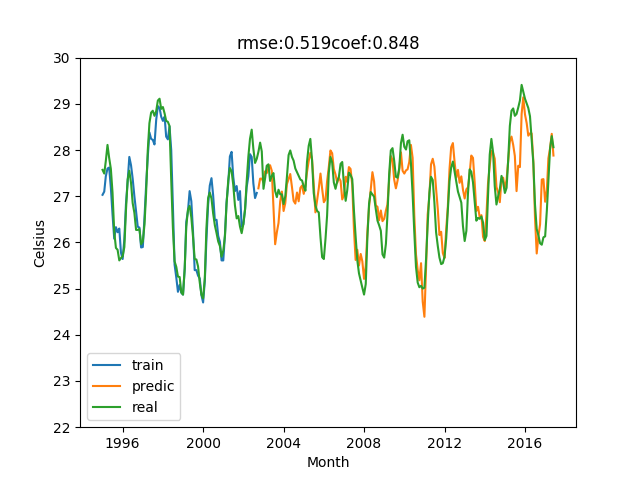
\includegraphics[scale=0.4]{figures/all_naive_5.png}
\caption{lead month=5时集成结果}
\end{minipage}
\begin{minipage}[t]{0.48\textwidth}
\centering
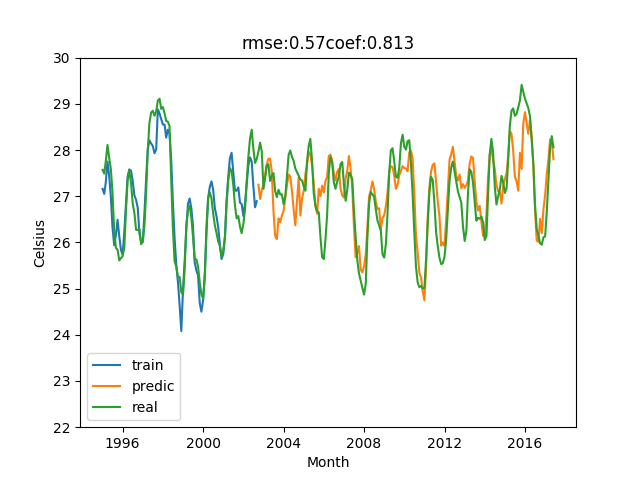
\includegraphics[scale=0.4]{figures/all_naive_6.png}
\caption{lead month=6时集成结果}
\end{minipage}
}
%\end{figure}
%\begin{figure}[H]
\subfigure{
\begin{minipage}[t]{0.48\textwidth}
\centering
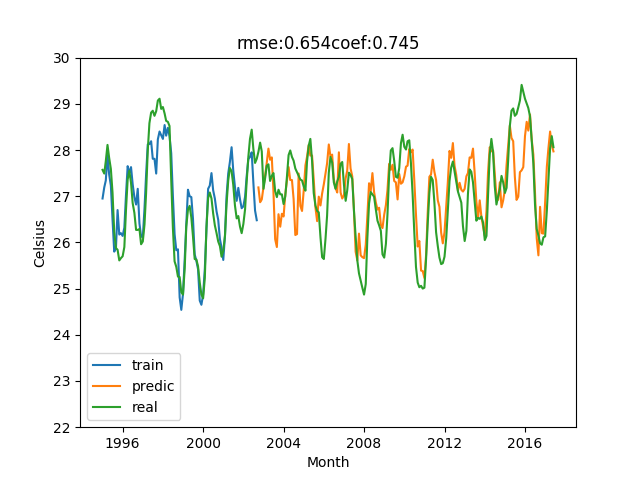
\includegraphics[scale=0.4]{figures/all_naive_7.png}
\caption{lead month=7时集成结果}
\end{minipage}
\begin{minipage}[t]{0.48\textwidth}
\centering
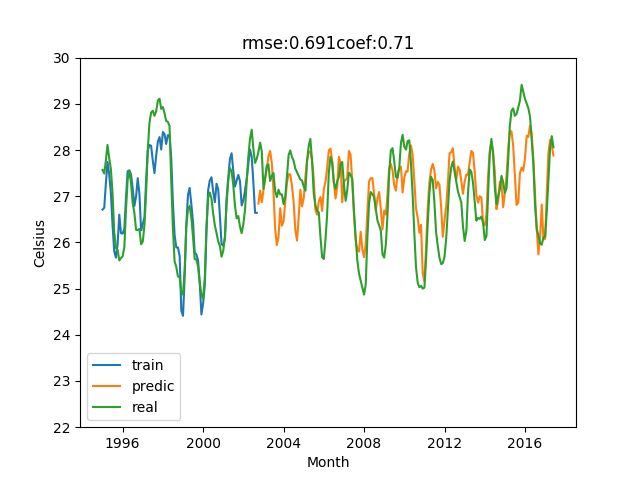
\includegraphics[scale=0.4]{figures/all_naive_8.png}
\caption{lead month=8时集成结果}
\end{minipage}
}
\end{figure}

从图中可以看出不同lead month的SST测试数据的RMSE都在1以下,且相关系数都在70\%以上。

为了方便与原来的集合平均的结果进行比较。图~\ref{fig:ml integration}展示了集合平均集成方法与本文的集合集成方法的不同lead month的平均集成结果。 由图可知,新提出的集合集成方法很大程度上改进了原方法,提高了模式集合输出数据的利用率。在RMSE结果上,不同lead month的平均改进结果高达32\%,充分说明了4.2节中方法的有效性。

 \begin{figure}[H] % use float package if you want it here
\label{prectresult}
  \centering
  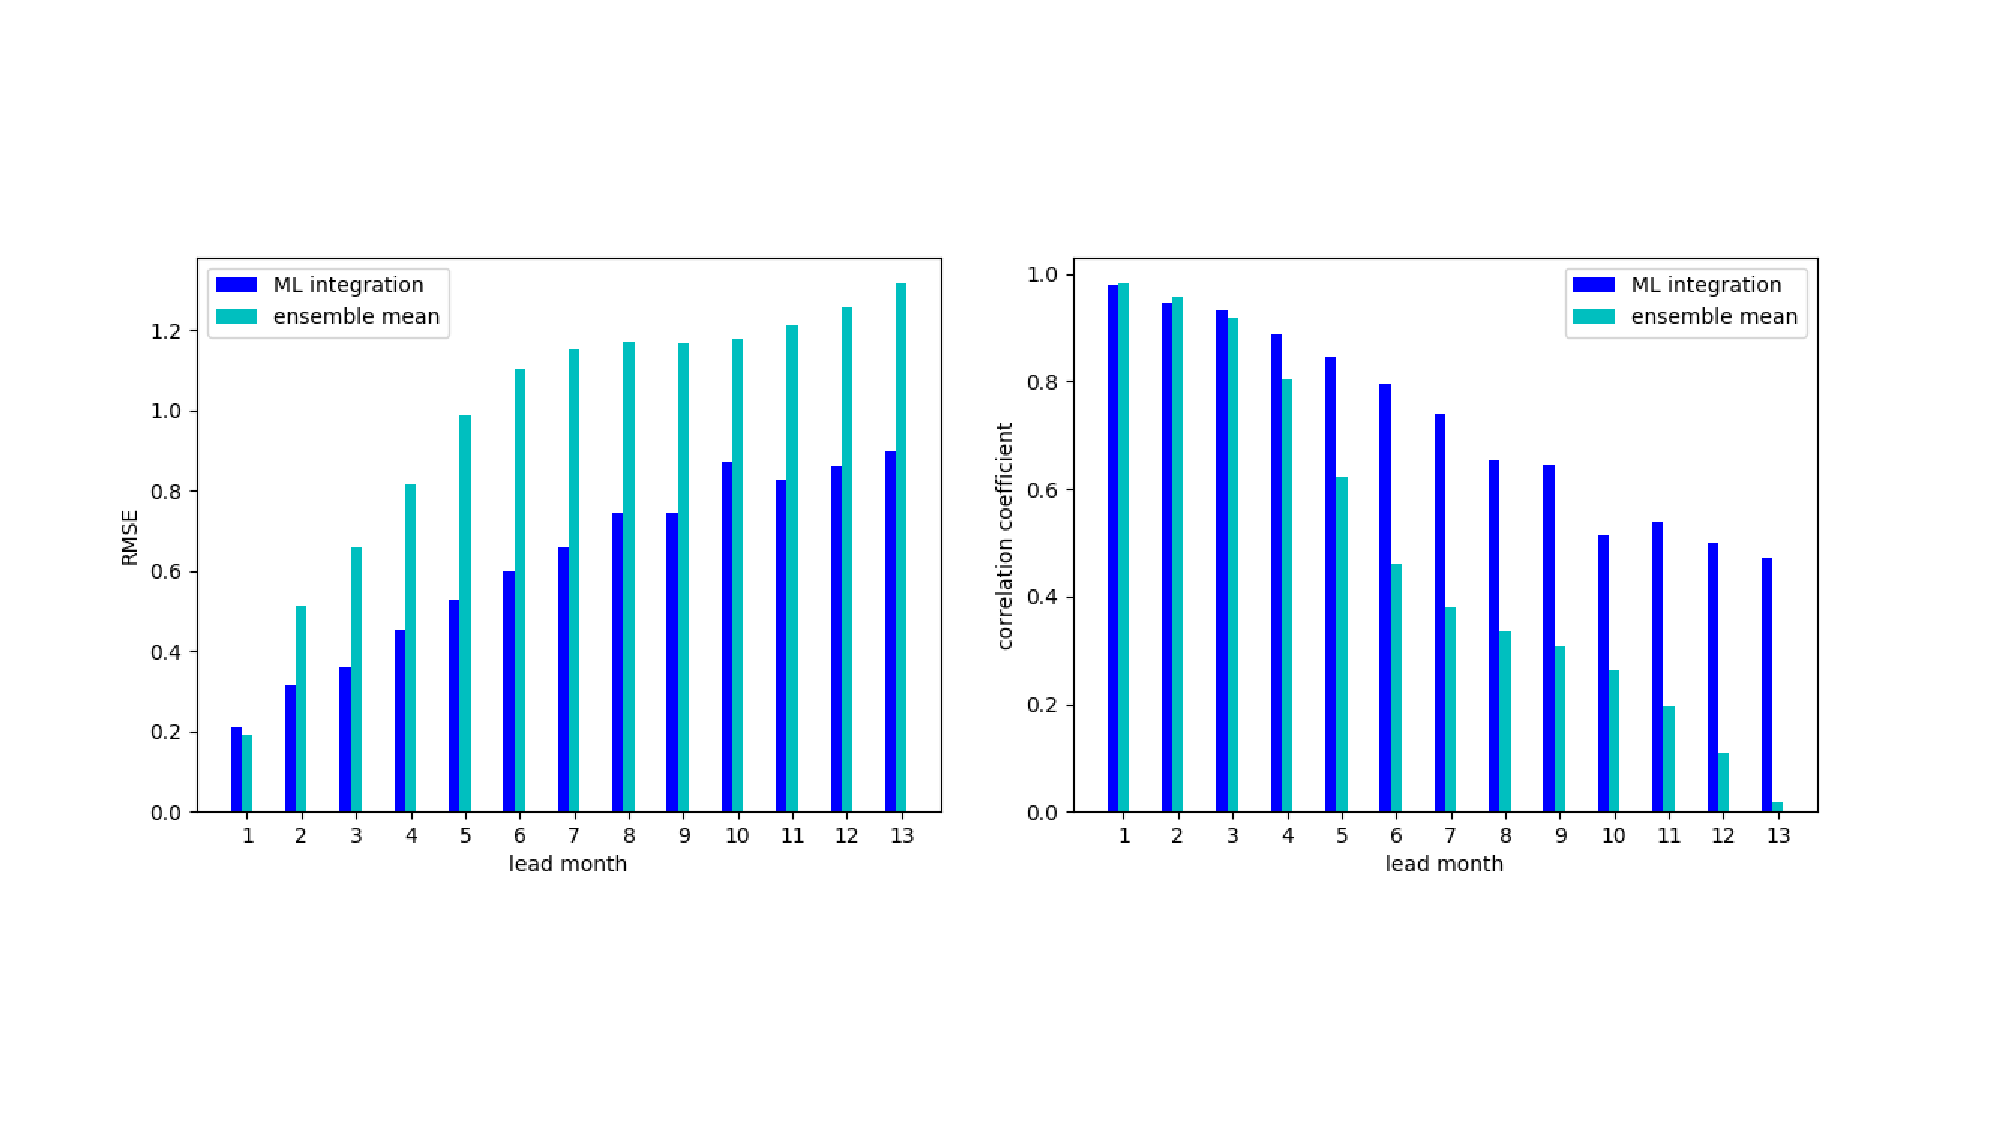
\includegraphics[scale=0.53,trim=55 90 0 100,clip]{figures/RMSEandcorr-ensega.pdf}
  \caption{机器学习修正方法与集合平均集成结果对比}
  \label{fig:ml integration}
\end{figure}

\section{本章小结}
本章首先提出了一种结合参数优化的气候系统模式的集合预测方法,另外为了进一步研究如何提升确定性集合预报能力,提高对集合成员数据的利用率,本章设计了一种基于机器学习的确定性集合集成方法。最后本章根据前文所述内容设计了综合集合预测系统。此系统包括了气候系统模式的参数优化流程和气候预测集合扰动的生成及集合评价技术等。将繁重的参数优化和集合扰动生成及预测过程自动化,为后续气候预测技术的研究提供了良好的试验平台。

为了验证上述方法有效性和系统的可用性,本章在BCC-CSM气候系统模式上做了降水集合预测试验以及ENSO集合集成试验。降雨预测试验结果表明本文中的集合预测方法对于确定性季节预报能力的提升十分明显。2008年12月到2009年3月全球降水MSE相对于LAF方法平均提升了15.1\%。ENSO预测试验集合集成方法对预报lead month为13个月的BCC-CSM气候系统模式输出的SST的结果修正效果明显。平均修正RMSE结果可相对于集合平均法提高32\%。